\section{Praktisch}

\begin{itemize}
	\item Gedeelde schijf:  \\	T:\textbackslash  IIWTCGMonitoraat \textbackslash  STEM\_gedeeld
	\item Toledo: inschrijven op community Ind. Ing. Gent en op community monitoraat
	\item Software: (zie ook Toledo)
	\begin{itemize}
		\item LaTex: TexStudio		
		\item Studenten leren wekren met Maple, Autocad, Solidworks
		\item Grafische software, indien interesse: Inkscape, GIMP, Blender.  
		\end{itemize}
\end{itemize}

\subsection*{Wie is wie}

\begin{itemize}
	\item Lieven De Strycker
	\item Dorine Bruneel
 \end{itemize}

\newpage

\section{Monitoraat en studiebegeleiding}

\subsection*{Wie is wie}

\begin{itemize}
	\item Tony Stevens
	\item Luc Demaegd
	\item Dimitri Coppens
\end{itemize}
Opm.: Sarah Detremmerie, Stuvo  
\subsection{Werking}
\begin{itemize}
	\item Student die binnenkomt op monitoraat krijgt steeds voorrang op andere taken (een student hoeft in principe geen afspraak te maken)
	\item In de mate van mogelijke: mails van studenten trachten te beantwoorden binnen 24u
	\item Testen: \begin{itemize}
		\item Eerste semester: partiële examens:  worden verbeterd door docenten zelf. Maandag 5 november: Algebra, Computers en Programmeren, dinsdag 6 november: Fysica 1, Chemie 1
		\item Tweede semester: monitoraatstesten: worden verbeterd door monitoren		
	\end{itemize}\end{itemize}
\subsection{Vakinhoudelijke begeleiding}
\emph{\hl{Vak waarvoor er momenteel maar \'e\'en begeleider is.}}
\begin{table}[H]\footnotesize
	\centering	
	\begin{tabular}{ lll}	
		\emph{Eerste semester} &  \\ 
		\hline
		Algebra & Luc Demaegd \\
		& Dimitri Coppens \\
		Analyse 1 & Luc Demaegd \\
		& Dimitri Coppens \\
		\hl{Chemie 1} & Luc Demaegd\\
		\hl{Fysica 1}& Tony Stevens   \\
		Mechanica 1 (Statica)& Tony Stevens\\
		& Luc Demaegd\\
		\hl{Computers en Programmeren}& Dimitri Coppens \\
		Materiaalkunde & \\
		\\
		 
		 \emph{Tweede semester}\\
		\hline
		\hl{Elektriciteit} & Tony Stevens \\
		Analyse 2 & Luc Demaegd \\
& Dimitri Coppens \\
\hl{Chemie 2} & Luc Demaegd\\
\hl{Fysica 2}& Tony Stevens   \\
Mechanica 2 (Dynamica )& Tony Stevens\\
& Luc Demaegd\\
\hl{Netwerken en Objectori\"entatie} & Dimitri Coppens 
		\end{tabular}
\end{table}



\subsection{Studiemethode- en planning, vorming}
Opleidingen, Joke Vanhoudt, werkgroep Associatie, Johan Declerck (studieloopbaanbgeleiders)
\section{Stuur- en werkgroepen}
\begin{itemize}
	\item Werkgroep Instroombegeleiding
	\item Overleg PR 
	\item STEM-coördinatie Associatie KU Leuven
\end{itemize}

\section{\link{https://iiw.kuleuven.be/toekomstigestudenten/mooc-wiskunde}{MOOC} \& zomercursus }

hardcopy: TexStudio, vertrekkende van format als Junior College en Innovation lab
\section{Contacten met secundaire scholen}
\begin{itemize}
	\item Don Bosco Zwijnaarde
	\item Don Bosco Sint-Denijs Westrem
	\item Edugo (Oostakker)
	\item Sint-Bavocollege (Natasha Ghesquière)
	\item Sint-Lievens
	\item Sint-Pietersinstituut
	\item \ldots
\end{itemize}


\newpage

\section{STEM}

\subsection{Associatie}
\link{http://www.stemvoorleerkrachten.be/}{website stuurgroep}

\begin{itemize}	
	\item Wim Dehaene
	\item Stefaan Vaes
	\item Katrien Kolenbergh, Katlijn Vangilbergen	
\end{itemize}


%\includegraphics[width=\textwidth]{transitieEducatiefAanbod_JC_InnovLab.jpg}
\subsection{Workshops}

\begin{itemize}
	\item brochure faculteit
	\item An De Vuyst
	\item Martha Houwen
\end{itemize}
\subsection{Specifieke lerarenopleiding}
Coördinatie: Johan Van den Bossche en Guy Durinck
\begin{itemize}
	\item FLACRA: zie bijlage
	\item Passief wonen
	\item Hydraulische arm + arduino/rasperry pi \& stepper of servo motortjes (lineaire actuator: goniometrie, radiaalbegrip,\ldots )
	\item Hovercraft: bluetooth, smartphone , cfr. infra.
	\item Luc Pinoy: Fosfaten, zie ook bijlage. 
\end{itemize}
\subsection{KU Leuven: Junior College en Innovation Lab}

%\subsection*{Wie is wie}

\begin{itemize}
	\item Stefaan Vaes, Jonas Kaerts
	\item Katrien Kolenbergh, Katlijn Vangilbergen
	\item Katrien Van Nimmen, Klaus, Peter Van den Broeck, Stef Pillaert
\end{itemize}
\subsubsection{Junior College}

\link{https://www.kuleuven.be/onderwijs/juniorcollege}{Bestaande Junior Colleges}
\begin{figure}[H]
	\centering	\includegraphics[width=0.4\textwidth]{cover_buigen_beven_basten}
\end{figure}


\begin{itemize}
	\item concept: syllabus, lessenreeks  
	\item opleiding voor leerkrachten 
	\item Huisstijl Junior College	 	
	\item \link{https://www.kuleuven.be/onderwijs/juniorcollege/jcdag}{Junior College Dag}8 januari 2019	
\end{itemize}

\subsubsection{Innovation Lab}
\link{https://eng.kuleuven.be/innovationlab}{Bestaande innovation labs}


\begin{figure}[H]
	\centering     %%% not \center
	\subfigure[Figure A]{\label{fig:koffer}\includegraphics[width=45mm]{innovation_lab_koffer}}
	\subfigure[Figure B]{\label{fig:b}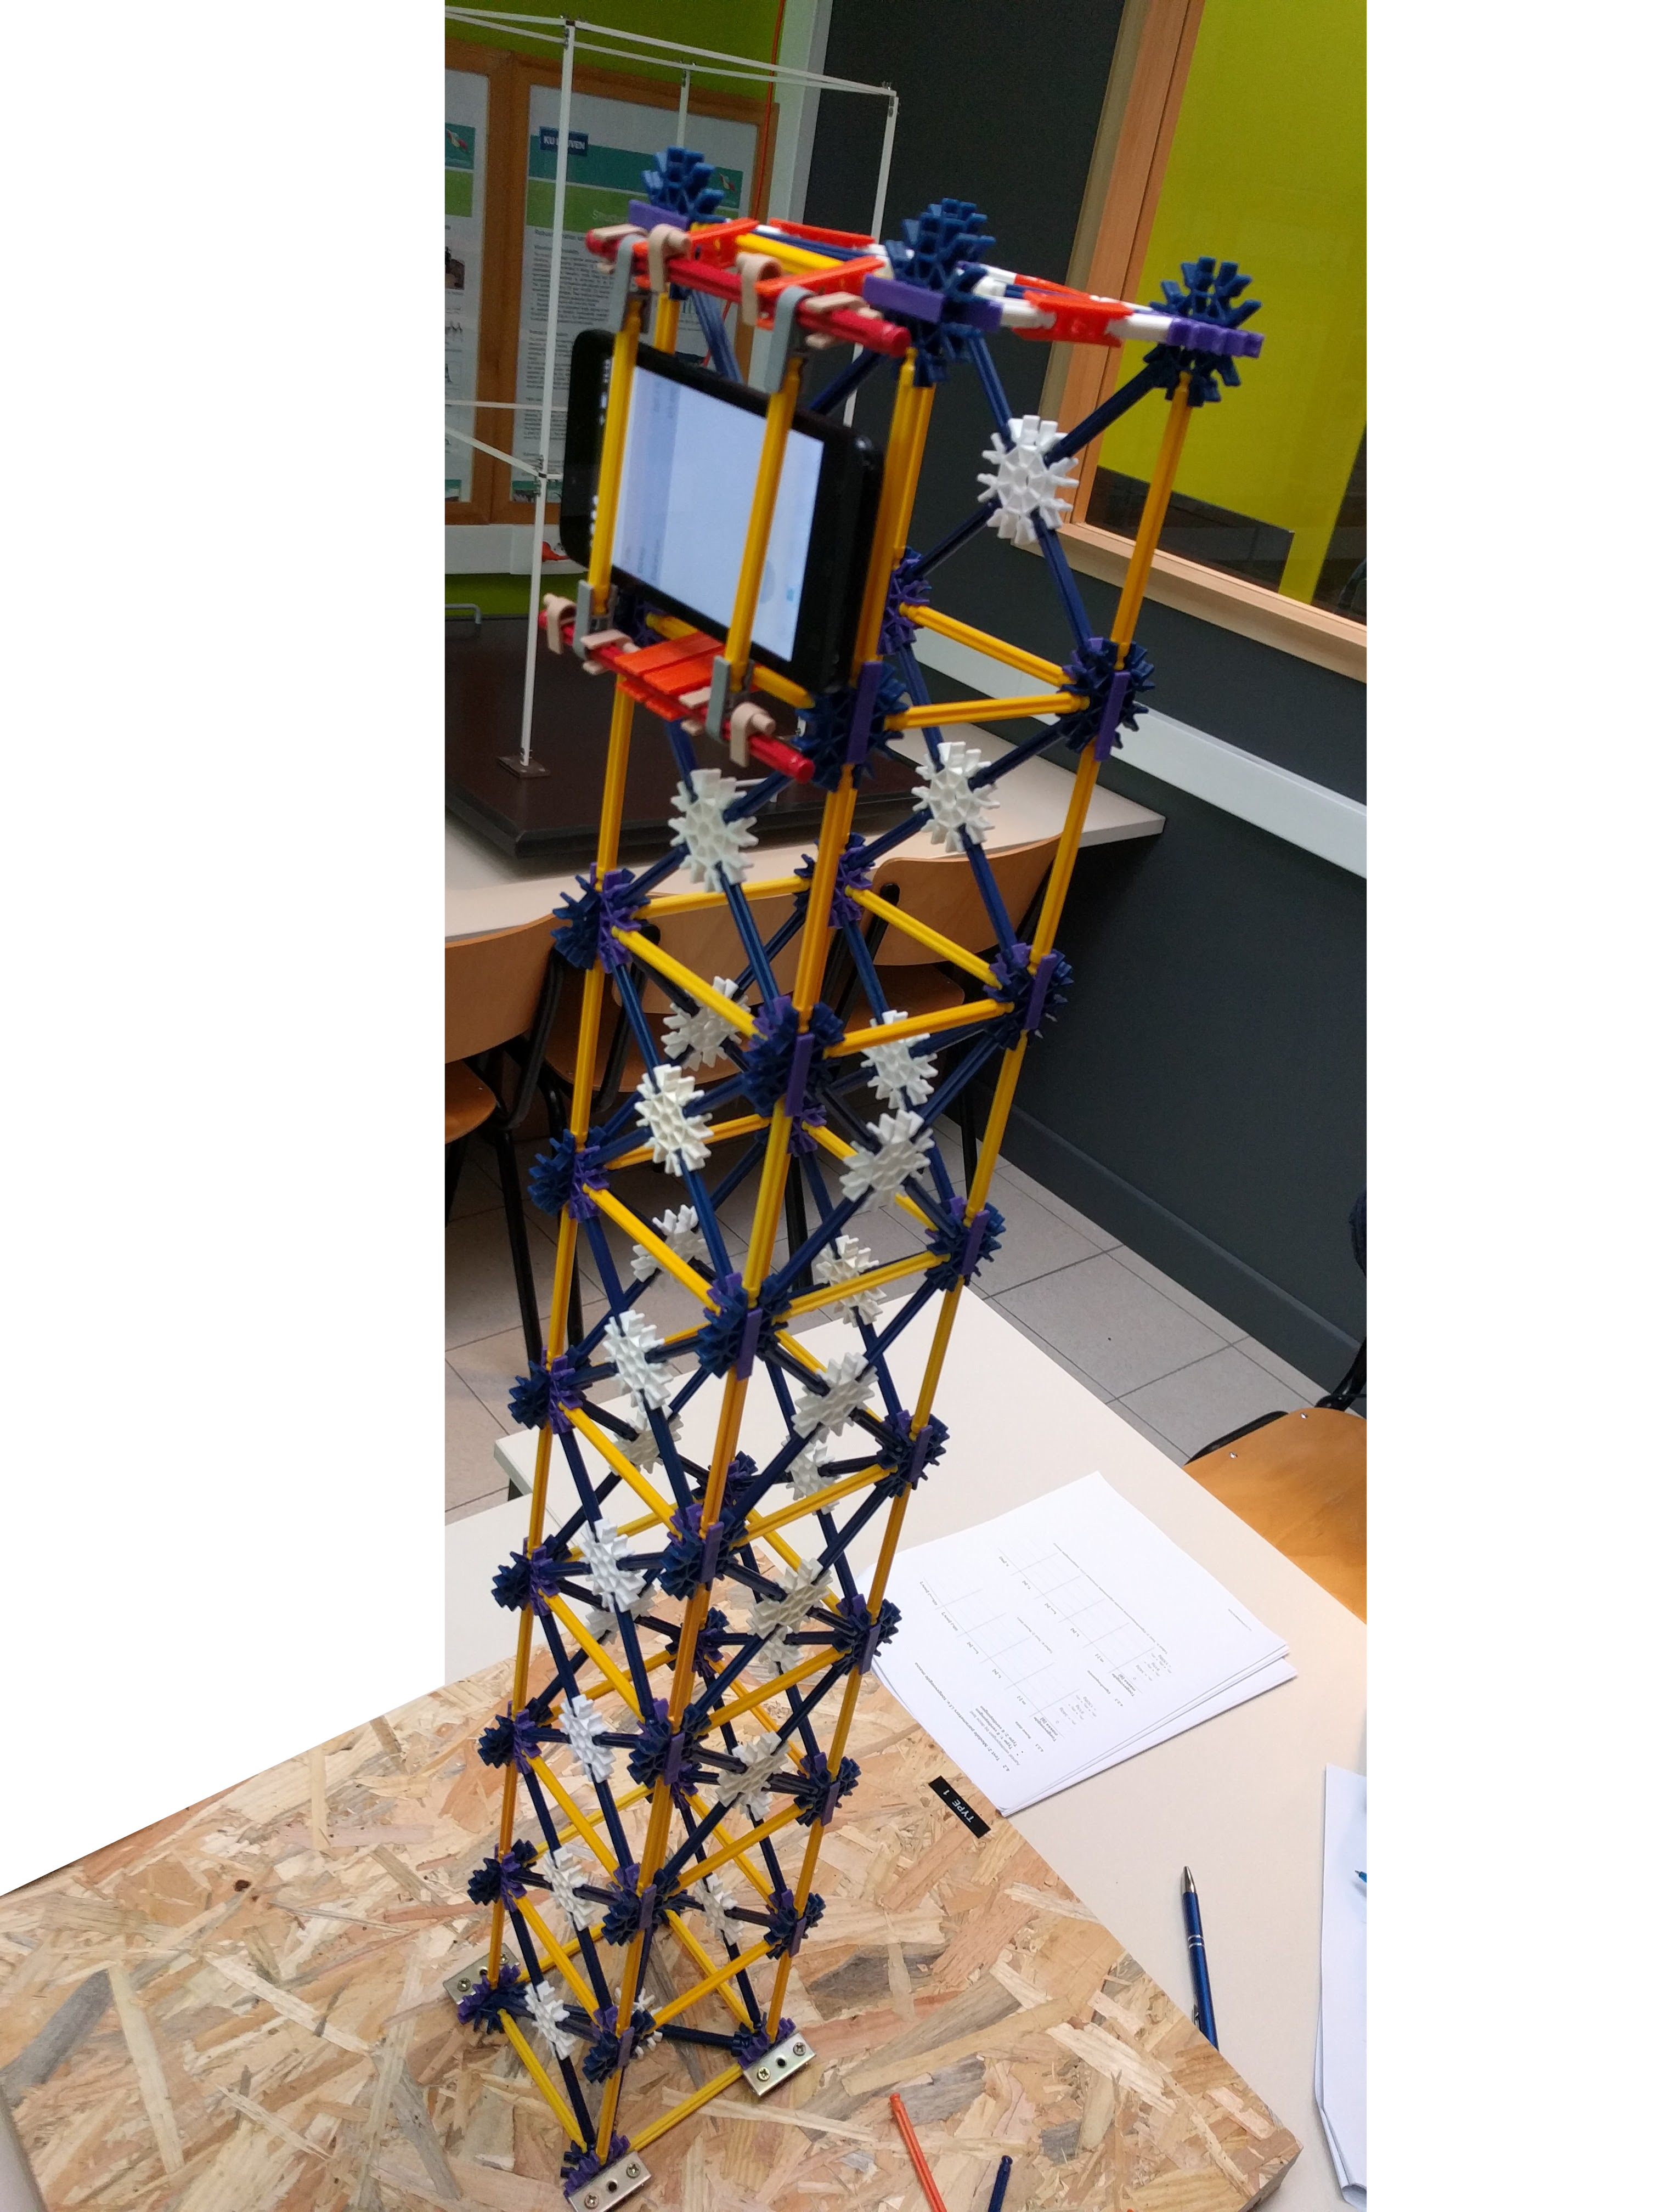
\includegraphics[width=60mm]{knex}}
	\caption{Innovation lab koffers en Knex toren}
\end{figure}




\begin{itemize}	
	\item concept: practicum, koffers
	\item opleiding voor leerkrachten 
	\item Huisstijl Innovation Lab
	
\end{itemize}

\subsection{Projecten}
Ieder project uit te werken i.s.m. leerkrachten en/of feedback vragen. Mogelijk om uit te bouwen tot Innovation Lab voor derde / tweede / eerste graad? 
\begin{itemize}	
	\item FLACRA: zie bijlage
	\item \link{https://www.youtube.com/watch?v=XTxCpTwFdOI}{Hydraulische arm}	
	\item[$\rightarrow$] Dag Van De Wetenschap 25 november 
	\begin{figure}[H]
		\centering
	\includegraphics[width=0.4\textwidth]{hydraulische_arm}	\end{figure}
	\item 	\link{https://www.youtube.com/watch?v=EtbyppA_BJU}{Hydraulische pers}
	\begin{figure}[H]
		\centering	\includegraphics[width=0.4\textwidth]{hydraulische_pers_asterechnics(3)}
	\end{figure}
	\item Hovercraft: \link{https://www.instructables.com/id/EAL-Arduino-Hovercraft/}{Arduino met bluetooth module, smartphone: App Inventor}
	\link{http://ai2.appinventor.mit.edu/?locale=en}{App Inventor}
	
	\begin{figure}[H]
	\centering
	\includegraphics[width=0.4\textwidth]{99hovercrafts(30).jpg}
	\end{figure}
	
	\item \link{https://www.youtube.com/watch?v=DfznnKUwywQ&t=12s}{Ingenieur voor één dag}
	\begin{figure}[H]
		\centering	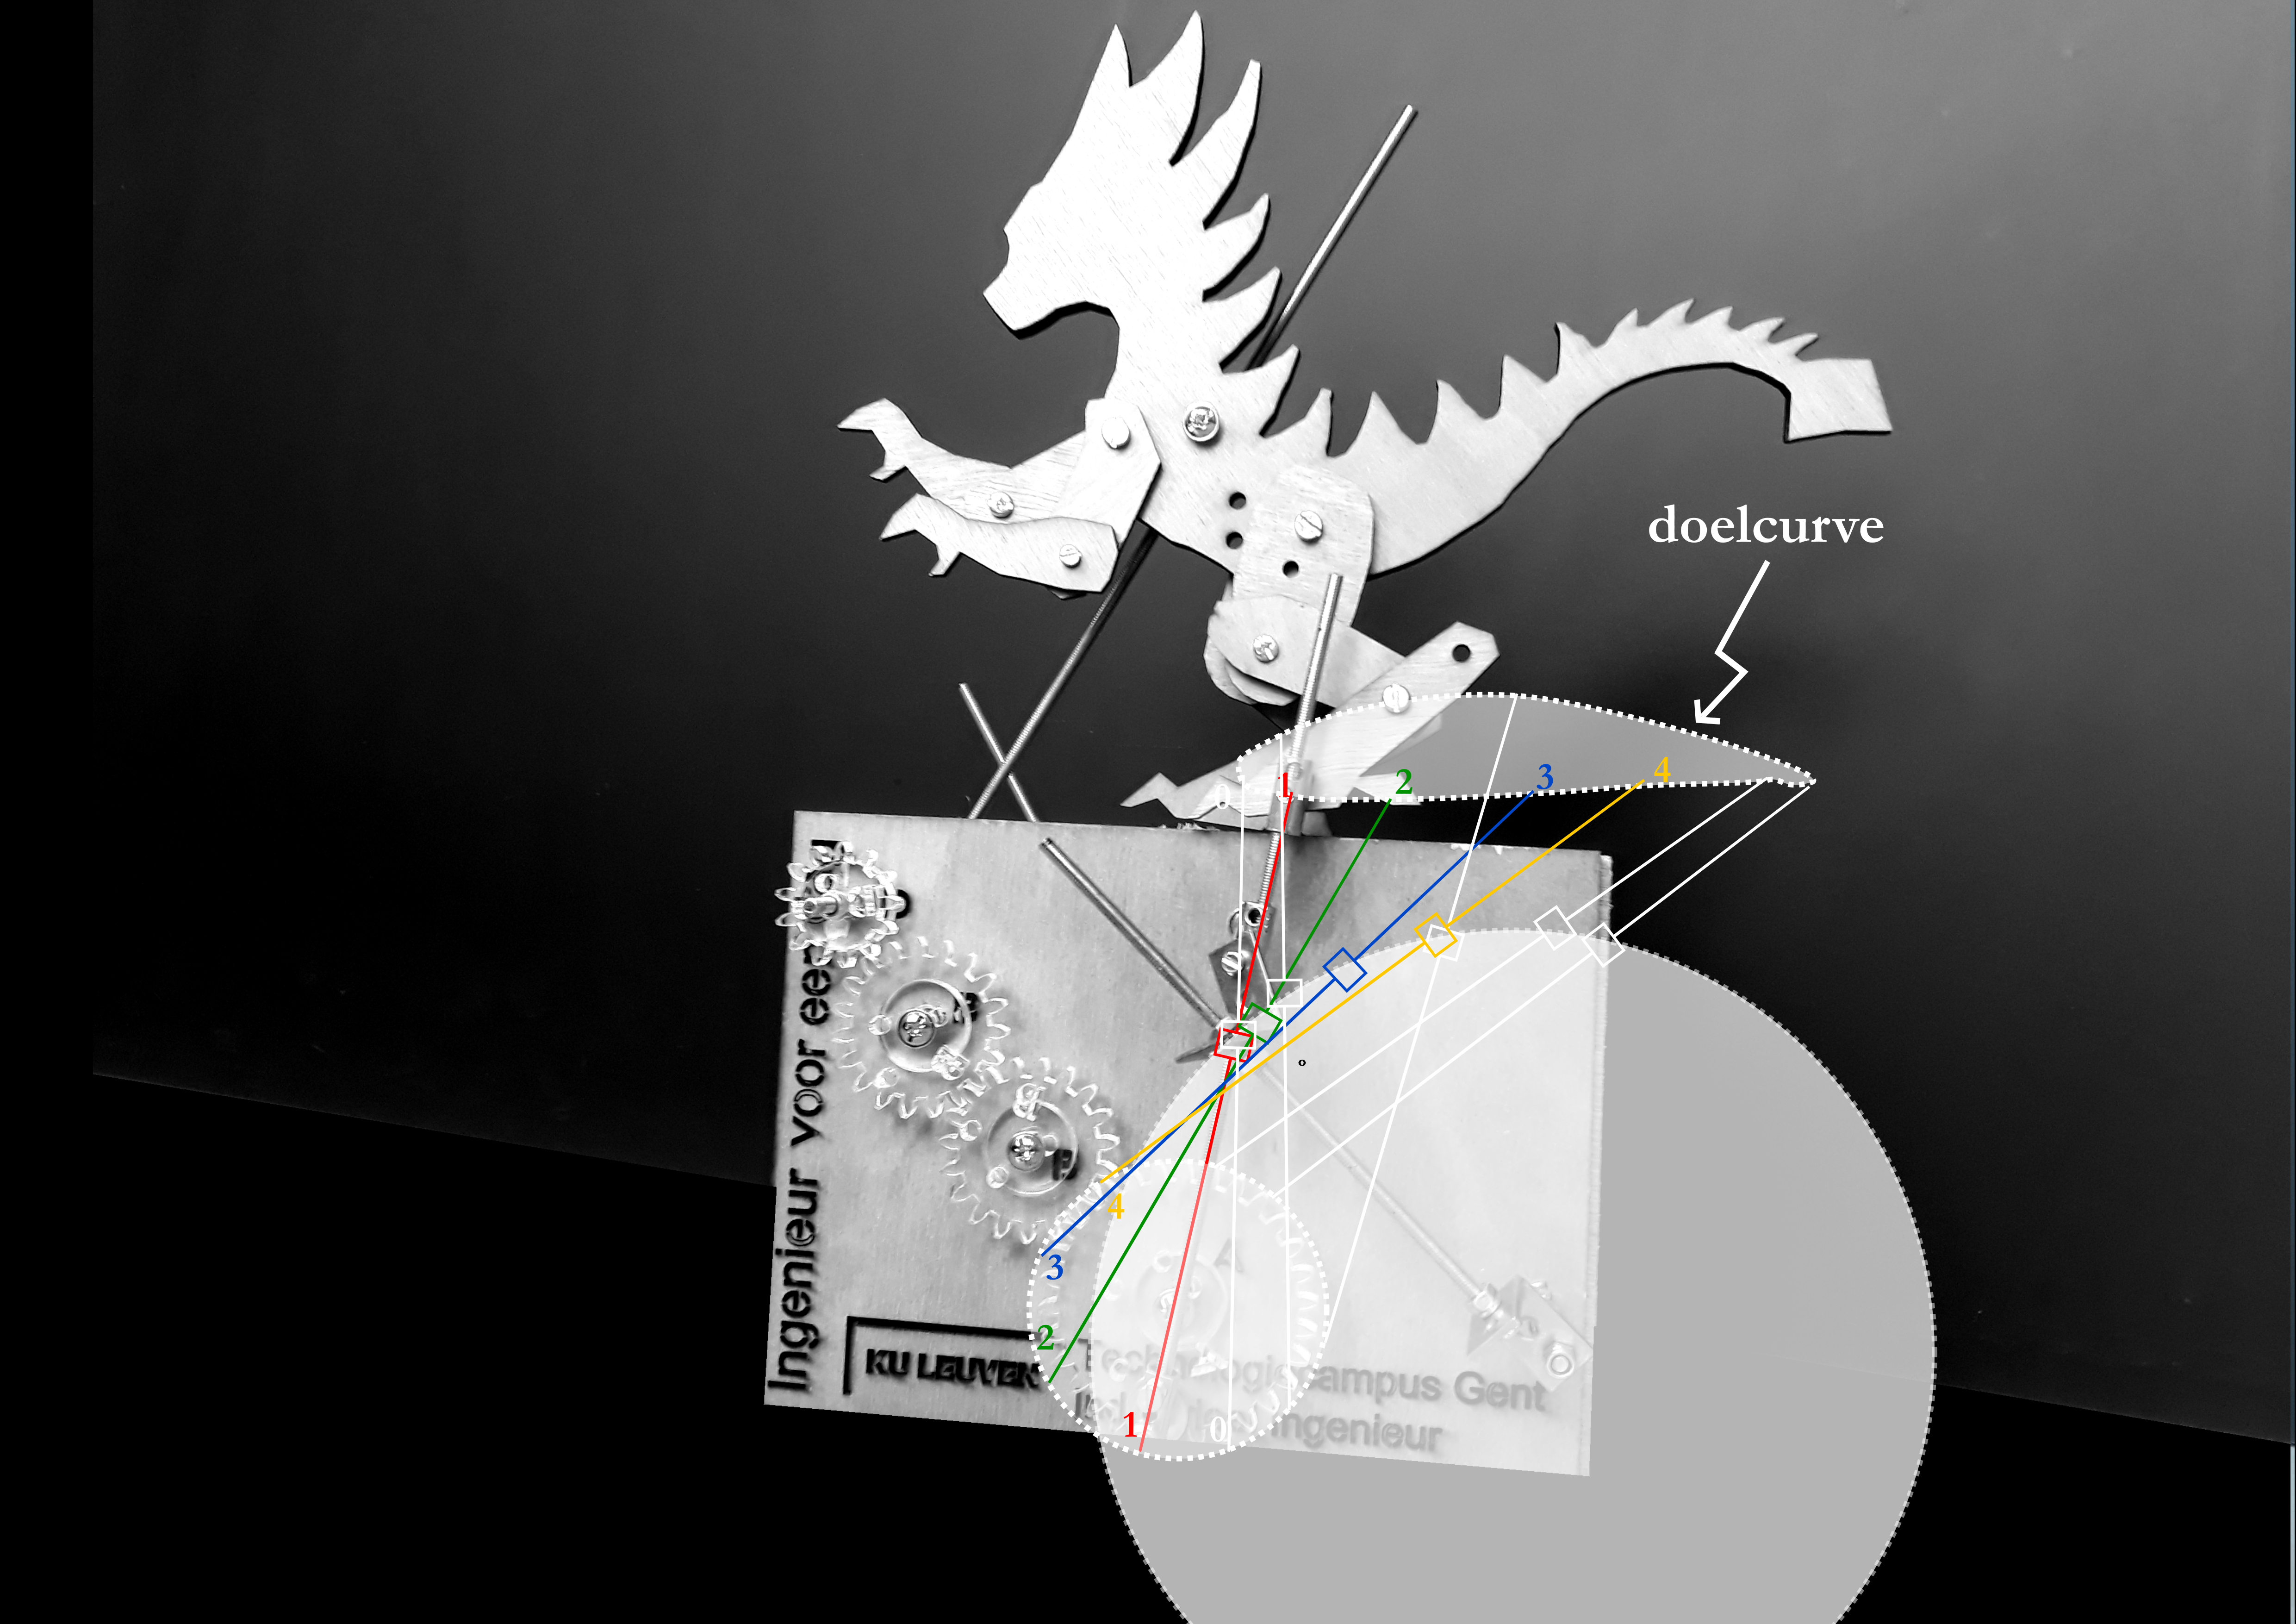
\includegraphics[width=0.4\textwidth]{ingenieur_voor_een_dag_foto_brochure}
	\end{figure}	
	\item \link{https://www.youtube.com/watch?v=1tXud_ugULc}{Elektromagnetische pen}, zie ook bijlage
\end{itemize}

\section{Varia}
\begin{itemize}
	\item Trotec lasercutter (DND lab)
	\item 3D printer
\end{itemize}

\section{Bijlages}
\includepdf[pages=-]{elektromagnetischePen180613.pdf}
\includepdf[pages=-]{FLACRA}
\includepdf[pages=-]{ingenieurVoorEenDag_180502}
\includepdf[pages=-]{Innovation_Lab_Fosfaat}
\includepdf[pages=-]{hydraulischeArmJarnoSander}
%\includepdf[pages=-]{vacature_monitoraat_en_STEM.PDF}
\includepdf[pages=-]{mooc_stem_1}
\includepdf[pages=-]{mooc_stem_2}